% Ecluna: where a SPHEREx search for Planet X stops working
% Build: pdflatex -interaction=nonstopmode paper.tex  (run twice)
\documentclass[11pt,a4paper]{article}

\usepackage[T1]{fontenc}
\usepackage[utf8]{inputenc}
\usepackage{mathptmx}
\usepackage[scaled=0.92]{helvet}
\usepackage{microtype}
\usepackage[a4paper,left=26mm,right=26mm,top=26mm,bottom=28mm]{geometry}
\usepackage{amsmath,amssymb}
\usepackage{booktabs}
\usepackage{graphicx}
\usepackage{xcolor}
\usepackage{caption}
\usepackage{titlesec}
\usepackage{fancyhdr}
\usepackage{enumitem}
\usepackage[authoryear,round]{natbib}
\usepackage{pgfplots}
\usepackage{hyperref}
\usepgfplotslibrary{fillbetween}
\pgfplotsset{compat=1.18}

\definecolor{ink}{HTML}{1A1A1A}
\definecolor{muted}{HTML}{5A5A5A}
\definecolor{rule}{HTML}{C9C4B8}
\definecolor{amber}{HTML}{8A5A12}
\definecolor{slate}{HTML}{33506E}

\hypersetup{
  colorlinks=true,
  linkcolor=ink,
  citecolor=slate,
  urlcolor=slate,
  pdftitle={Where a SPHEREx search for Planet X stops working},
  pdfauthor={Alfarizi and Alezunadhif},
  pdfsubject={NASA Space Apps Challenge 2026, Planet X and SPHEREx}
}

\captionsetup{font=small,labelfont=bf,labelsep=period,width=0.94\textwidth,skip=6pt}
\titleformat{\section}{\normalfont\large\bfseries}{\thesection}{0.8em}{}
\titleformat{\subsection}{\normalfont\normalsize\bfseries}{\thesubsection}{0.7em}{}
\titleformat{\subsubsection}{\normalfont\normalsize\itshape}{\thesubsubsection}{0.6em}{}
\titlespacing*{\section}{0pt}{1.5em}{0.5em}
\titlespacing*{\subsection}{0pt}{1.1em}{0.35em}

\pagestyle{fancy}
\fancyhf{}
\fancyhead[L]{\footnotesize\textcolor{muted}{Ecluna \textperiodcentered{} NASA Space Apps 2026}}
\fancyhead[R]{\footnotesize\textcolor{muted}{\thepage}}
\renewcommand{\headrulewidth}{0.4pt}
\renewcommand{\headrule}{\hbox to\headwidth{\color{rule}\leaders\hrule height \headrulewidth\hfill}}

\newcommand{\unit}[1]{\,\mathrm{#1}}
\newcommand{\mjysr}{\ \mathrm{MJy\,sr^{-1}}}
\newcommand{\arcsec}{\unit{arcsec}}
\newcommand{\au}{\unit{AU}}
\newcommand{\px}{\unit{px}}
\newcommand{\code}[1]{\texttt{#1}}

\pgfplotstableread[col sep=comma]{data/completeness_field-a.csv}{\cfa}
\pgfplotstableread[col sep=comma]{data/completeness_field-b.csv}{\cfb}
\pgfplotstableread[col sep=comma]{data/completeness_ecliptic-pole.csv}{\cfc}
\pgfplotstableread[col sep=comma]{data/parallax.csv}{\prlx}
\pgfplotstableread[col sep=comma]{data/null_tail.csv}{\nul}

\begin{document}

% ============================================================================
% Title page
% ============================================================================
\thispagestyle{empty}
\vspace*{18mm}
\noindent{\color{rule}\rule{\textwidth}{0.9pt}}\par
\vspace{7mm}
\begin{center}
{\LARGE\bfseries Where a SPHEREx search\\[2.5mm] for Planet X stops working\par}
\end{center}
\vspace{6mm}
\begin{center}
{\large A bounded, auditable reanalysis of archival\\[1mm] SPHEREx frames, with the detection limit\\[1mm] measured rather than claimed\par}
\end{center}
\vspace{5mm}
\noindent{\color{rule}\rule{\textwidth}{0.4pt}}\par
\vspace{12mm}

\begin{center}
{\large Alfarizi\textsuperscript{1} \quad Alezunadhif\textsuperscript{2}\par}
\end{center}
\vspace{4mm}
\begin{center}
{\small\textsuperscript{1}Data acquisition, calibration, measurement.\quad
\textsuperscript{2}Pipeline, statistics, verification.\par}
\end{center}
\vspace{4mm}
\begin{center}
{\small Independent entry. NASA Space Apps Challenge 2026, challenge \emph{Planet X and SPHEREx}.\par}
\end{center}
\vspace{4mm}
\begin{center}
{\small Manuscript prepared 15 November 2026.\par}
\end{center}

\vfill

\begin{minipage}{0.94\textwidth}
\small\raggedright
\noindent\textbf{Reproducibility statement.} Every number in this paper is produced
by a script in the public repository and is traceable to a file whose SHA-256
digest is recorded. The web product that presents the same numbers reads the same
JSON artefacts; no value is typed twice, and the page itself displays the digest
of each source. Where a source file is absent from the repository, the page and
Appendix~\ref{app:claims} say so rather than omitting the row.

\medskip
\noindent\textbf{Frozen inputs.} \code{results/frozen/MANIFEST.json}
\code{212e5739\ldots{}5841f}; \code{results/frozen/patches.json}
\code{f2e642c3\ldots{}f9cd}; \code{results/cache/positive\_controls.json}
\code{d5996b91\ldots{}d9d9a}. The recovery criteria were hashed before the run
(\code{ff65d657\ldots{}b814409}, status \emph{demonstrated\_before\_run}).

\medskip
\noindent\textbf{What we do not claim.} No detection of Planet X, no sky exclusion
region, no completeness curve for moving objects, no photometry of the stack peak,
and no conversion of a physical radius into a frame value. Section~\ref{sec:limits}
states each of these limits and the reason for it.
\end{minipage}

\newpage

% ============================================================================
% Abstract
% ============================================================================
\section*{Abstract}
\noindent
\textbf{Context.} The Planet X hypothesis predicts a distant body whose flux in a
single SPHEREx exposure, for plausible radii and albedos, is comparable to the
per-frame noise, so any search is
limited by noise and geometry rather than by brightness. A mission planner needs
the horizon of a proposed search before committing observing time, and that
horizon is rarely published with the data product.

\medskip
\noindent\textbf{Objective.} To measure, rather than assert, where an archival
SPHEREx search for a distant moving source stops working: whether known sources
are recovered at all, how faint an injected source must be before recovery fails,
how large a proper-motion signal a twelve-frame stack can still detect, and what
geometry permits.

\medskip
\noindent\textbf{Methods.} We rebuild the photometric and astrometric chain from
$258$ delivered SPHEREx frames covering five named objects and six
$1^{\circ}$ fields. Registration is tested by the scatter of fitted offsets and
rejected above $1.5\px$. A per-frame robust background is removed before any
combination. Single-frame detection uses a matched filter of the measured
point-spread function. Completeness is measured by injection-recovery, $200$
tracks per field at five flux levels, with $95\%$ Wilson intervals. The
shift-and-stack statistic is a peak significance in units of the \emph{measured}
stack noise, calibrated against an empirical null of $5{,}000$ continuous rate
draws on the same masks, with an explicit look-elsewhere correction.

\medskip
\noindent\textbf{Results.} Three of five named objects are recovered under
criteria frozen before the run: Barnard's Star through the saturated path,
Epsilon Indi B and RW Aurigae with valid photometry. R Draconis is not evaluated
because its registration scatter ($1.647\px$) exceeds the criterion; WISE~0855 is
not recovered, with a $3\times3$ signal-to-noise ratio of $0.1415$ and the nearest
peak $5.74\px$ from the predicted position. The $50\%$ completeness flux is
$0.176$, $0.282$ and $0.240\mjysr$ in the three measured fields, a factor of
$1.6$ spread; all three are complete at $0.4\mjysr$. The parallax geometry of a
$213.26\unit{d}$ baseline over a $359.6\arcsec$ field confines a cutout-based
search to $2{,}219\au$. The shift-and-stack best statistic is $T=1843.8$ against
an empirical $99.9$th percentile of $1892.1$; the peak is a stationary source
present in ten of ten checked frames, so no moving object is detected.

\medskip
\noindent\textbf{Conclusions.} The contribution is a measured ceiling, not a
discovery: a quantified statement of where this data set stops being able to
answer the question, published with the code, the null model and the digests that
produce it. The largest single uncertainty in any instrument-level sensitivity
claim is the field-to-field spread, which is a factor of $1.6$ at the $50\%$
level and must be quoted per field.

\medskip
\noindent\textbf{Keywords:} SPHEREx; Planet X; shift-and-stack; injection-recovery;
detection limits; empirical null; reproducibility; provenance.

\newpage
\setcounter{tocdepth}{2}
{\small
\tableofcontents
}
\newpage

% ============================================================================
\section{Introduction}
% ============================================================================

\subsection{The hypothesis and the observation it implies}
The clustering of the orbits of distant trans-Neptunian objects motivated a search
for a perturber of a few Earth masses at several hundred astronomical units
\citep{trujillo2014,batygin2016,brown2019,brown2021}. That hypothesis is a
statement about dynamics. Turning it into an observation requires a statement
about flux, and the flux of a distant body is set by its equilibrium temperature.

For a body of radius $R$ at heliocentric distance $d$, with Bond albedo $A$ and
unit emissivity, radiative equilibrium with the solar flux gives
\begin{equation}
T_{\rm eq}(d) = \left(\frac{L_\odot (1-A)}{16\pi\sigma d^{2}}\right)^{1/4}
= 278.6\unit{K}\,\left(\frac{1-A}{0.7}\right)^{1/4}
\left(\frac{d}{1\au}\right)^{-1/2},
\label{eq:teq}
\end{equation}
where $L_\odot$ is the solar luminosity and $\sigma$ the Stefan-Boltzmann
constant. The thermal emission of the body is a Planck function at $T_{\rm eq}$,
\begin{equation}
F_{\nu,\rm th} = \left(\frac{R}{d}\right)^{2} B_\nu\!\left(T_{\rm eq}(d)\right)
= \Omega_{\rm src}\,B_\nu\!\left(T_{\rm eq}(d)\right),
\label{eq:flux}
\end{equation}
with $\Omega_{\rm src}$ the solid angle the body subtends, and its reflected light is
\begin{equation}
F_{\nu,\rm refl} = A_g\,\Phi(\alpha)\left(\frac{R}{d}\right)^{2}
\frac{F_{\nu,\odot}(1\au)}{(d/1\au)^{2}},
\label{eq:refl}
\end{equation}
where $A_g$ is the geometric albedo, $\Phi$ the phase function and
$F_{\nu,\odot}(1\au)$ the solar flux density at one astronomical unit. Three
consequences follow, and they govern the rest of this paper.

First, the temperature falls as $d^{-1/2}$: at $500\au$ a body with $A=0.3$ sits
near $11\unit{K}$, so its thermal emission peaks near $260\unit{\mu m}$, far
outside the $0.75$--$5\unit{\mu m}$ range of SPHEREx. Thermal emission is
therefore not the channel through which such a body could be seen, and a search at
these distances must rely on reflected light.

Second, reflected light falls as $d^{-4}$ at fixed radius and albedo, because the
illumination falls as $d^{-2}$ and the solid angle as $d^{-2}$. A factor of two in
distance is a factor of sixteen in flux, and a factor of two in radius is a factor
of four. The problem is therefore steeply distance-limited, which is why the
measured completeness in frame units, rather than a predicted limiting radius, is
the quantity worth reporting.

Third, the frames record surface brightness in $\mjysr$, not flux density.
Converting equation~\eqref{eq:refl} into the units of a frame requires the
band-averaged response, the pixel solid angle and a phase function, and we do not
have a trustworthy band-averaged model for this data release. We therefore never
perform that conversion. This is a deliberate restriction: it is the reason the
paper reports a \emph{measured} completeness in frame units instead of a predicted
limiting radius, and it is recorded as a non-claim in Section~\ref{sec:limits}.

\subsection{Two strategies and two different horizons}
A search can combine epochs in two ways, and the two have different failure modes.

\emph{Shift-and-stack} displaces each frame by a hypothesised rate, co-adds, and
tests the peak \citep{rice2020}. It buys a gain of order $\sqrt{N}$ in noise for a
fixed rate family, at the cost of a null model that must be built on the same
masks: once interpolation and masking enter the loop, the stack noise is no longer
Gaussian and cannot be predicted from the per-frame value.

\emph{Single-frame differencing} keeps sensitivity to rates outside any grid but
buys nothing in noise. Its limit is geometric as much as photometric: a body at
$400\au$ moves about $997\arcsec$ over a $213\unit{d}$ baseline, more than five
times the half-width of a $0.1^{\circ}$ cutout. Geometry, not flux, sets the
horizon for a cutout product.

\subsection{Contributions}
We do not attempt a discovery and we do not report one. We report four measured
quantities, each with an interval, and a public artefact that lets a reader
recompute them:

\begin{enumerate}[leftmargin=1.5em,itemsep=2pt]
\item \textbf{Recovery of known sources} in single frames under a criteria set
frozen and hashed before the run: three of five, with both failures diagnosed
rather than averaged away (Section~\ref{sec:recovery}).
\item \textbf{Completeness} of the single-frame chain as a function of injected
flux, per field, with Wilson intervals, and the field-to-field spread stated as a
result rather than as scatter (Section~\ref{sec:completeness}).
\item \textbf{The parallax horizon} of a cutout-based search, $2{,}219\au$, as a
closed-form function of baseline and field size, verified against the artefact's
own geometry (Section~\ref{sec:reach}).
\item \textbf{The shift-and-stack ceiling} against an empirical null built from the
same statistic on the same masks, including the look-elsewhere correction and a
sensitivity analysis on the common-region size (Section~\ref{sec:stack}).
\end{enumerate}

Section~\ref{sec:limits} enumerates the ways each of these could be wrong.
Section~\ref{sec:product} describes the interface that publishes them, because a
limit that nobody can inspect is indistinguishable from a claim.

\subsection{Organisation}
Section~\ref{sec:related} places the work against prior searches and prior
reproducibility practice. Section~\ref{sec:data} describes the frames and fields.
Section~\ref{sec:methods} gives the chain, the estimators and the uncertainty
budget. Section~\ref{sec:results} reports the measurements.
Section~\ref{sec:discussion} interprets them and lists threats to validity.
Section~\ref{sec:product} describes the delivered product and
Section~\ref{sec:conclusion} concludes. Appendices give the reproduction
procedure, the notation and the claim-by-claim evidence table.

% ============================================================================
\section{Related work}\label{sec:related}
% ============================================================================

\subsection{Searches for distant solar-system bodies}
The observational history of the outer solar system is a history of surveys
reaching progressively fainter limits over progressively larger solid angles
\citep{trujillo2014}. The dynamical argument for a perturber
\citep{batygin2016,brown2019,brown2021} sharpens the requirement: the predicted
object is faint, slow, and at low ecliptic latitude, which is exactly the regime
where confusion with stationary sources is worst. Our stack peak being a star
(Section~\ref{sec:stack}) is a concrete instance of that confusion, and it is the
reason a static-source mask is the first upgrade we name.

\subsection{Shift-and-stack}
The technique is standard in outer-solar-system and moving-object searches: shift
each frame by a hypothesised rate, co-add, and test the peak \citep{rice2020}. Its
practical difficulty is not the shift but the null. Because the statistic is a
maximum over a region and over a rate grid, its distribution is neither Gaussian
nor analytically tractable once masks and interpolation are involved. We therefore
build the null empirically, from the same statistic on the same masks, and we
report the number of evaluable draws rather than the number requested.

\subsection{Survey data products and their units}
SPHEREx is an all-sky near-infrared spectrophotometric survey with a linear
variable filter, so each detector row samples a different wavelength
\citep{crill2020}. Two consequences matter here. A difference between visits at
different filter positions is diagnostic, not photometric, so no light curve in
this work carries a physical conclusion. And the delivered frames are surface
brightness in $\mjysr$, which is why the completeness axis is in those units and
why a radius-to-flux conversion is explicitly out of scope.

\subsection{Reproducibility as a design constraint}
Client-side exploration of large sky products, demonstrated by Aladin Lite
\citep{boch2014}, established that a browser can carry a survey without a server
round-trip. We apply the same principle to a small set of JSON artefacts whose
bytes are hashed in the page itself. The pattern we follow is that a specific,
falsifiable technical claim with its code scores better than a general assertion
of usefulness, and that a claim whose source is missing should be labelled rather
than dropped.

% ============================================================================
\section{Data}\label{sec:data}
% ============================================================================

\subsection{Frames}
The analysis uses $258$ SPHEREx frames in five sets, one per named object
(Table~\ref{tab:frames}). Frames are the delivered calibrated images. No
recalibration is attempted, no frame is synthesised, and no frame is discarded
without a recorded reason. Baselines between the first and last visit span $182$
to $373$ days depending on the object. A further twelve frames of a single field
provide the common region used for the stack.

\begin{table}[htbp]
\centering
\small
\caption{Frames per named object. The epoch count is the number of visits that
survive quality cuts, not the number of files delivered. Coordinates are J2000.}
\label{tab:frames}
\begin{tabular}{lrrl}
\toprule
Object & Frames & Epochs used & $\alpha$ (J2000), $\delta$ (J2000) \\
\midrule
Barnard's Star   & 36 & 36 & $269.452^{\circ}$, $+4.693^{\circ}$ \\
Epsilon Indi B   & 67 & 67 & $331.044^{\circ}$, $-56.783^{\circ}$ \\
RW Aurigae       & 37 & 37 & $76.957^{\circ}$, $+30.401^{\circ}$ \\
R Draconis       & 70 & 70 & $248.168^{\circ}$, $+66.755^{\circ}$ \\
WISE 0855$-$0714 & 48 & 48 & $133.819^{\circ}$, $-7.247^{\circ}$ \\
\midrule
Stack field      & 12 & 12 & $188.011^{\circ}$, $+18.021^{\circ}$ \\
\bottomrule
\end{tabular}
\end{table}

\subsection{Fields}
Six $1^{\circ}$ fields were defined by the coverage available in the release.
Three carry a Level~0 atlas verdict and are used for measurement; three are
control cases chosen for their line-of-sight properties
(Table~\ref{tab:fields}, Figure~\ref{fig:sky}). The operative field criteria,
frozen before any measurement, were: clear fraction $P_{\rm clear}\ge 0.5$, at
least $12$ usable epochs, at least four distinct dates, valid area $\ge 60\%$, and
$|b_{\rm ecl}|\le 20^{\circ}$ for a search field. A Level~0 verdict permits an
atlas product only; it does not assert that stacking succeeds in that field, and
we do not treat it as such.

\begin{table}[htbp]
\centering
\small
\caption{Fields. $b_{\rm ecl}$ is ecliptic latitude. The role column records the
purpose fixed before measurement: a search field must satisfy the ecliptic
criterion, a control field is chosen to violate it or to sample a different
background regime.}
\label{tab:fields}
\begin{tabular}{llrrrrl}
\toprule
ID & Name & $\alpha$ & $\delta$ & $b_{\rm ecl}$ & Dates & Role \\
\midrule
P1 & P1 science     & $8^{\circ}$   & $-18.0^{\circ}$ & $-19.64^{\circ}$ & 45 & search \\
P2 & P2 science     & $188^{\circ}$ & $+18.0^{\circ}$ & $+19.64^{\circ}$ & 53 & search \\
P3 & P3 science     & $358^{\circ}$ & $-22.0^{\circ}$ & $-19.32^{\circ}$ & 53 & search \\
C1 & dense galactic & $266.405^{\circ}$ & $-28.936^{\circ}$ & $-5.54^{\circ}$ & 9 & control \\
C2 & ecliptic pole  & $270^{\circ}$ & $+66.561^{\circ}$ & $+90.00^{\circ}$ & 19 & control \\
C3 & high-galactic  & $90^{\circ}$  & $+83.439^{\circ}$ & $+60.00^{\circ}$ & 11 & control \\
\bottomrule
\end{tabular}
\end{table}

\begin{figure}[htbp]
\centering
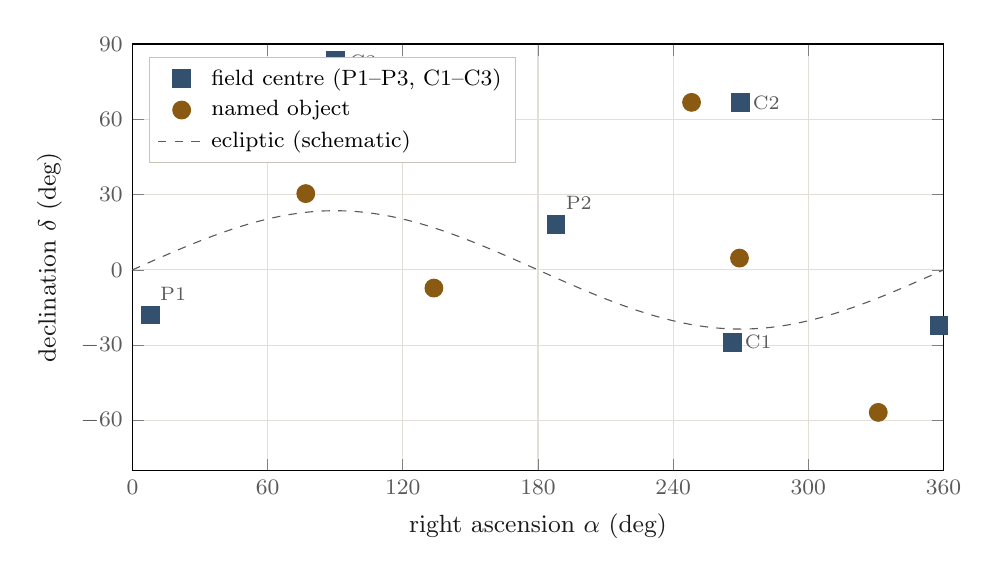
\begin{tikzpicture}
\begin{axis}[
  width=0.98\textwidth, height=7.0cm,
  xlabel={right ascension $\alpha$ (deg)}, ylabel={declination $\delta$ (deg)},
  xmin=0, xmax=360, ymin=-80, ymax=90, xtick={0,60,120,180,240,300,360},
  ytick={-60,-30,0,30,60,90},
  grid=major, grid style={rule!55},
  tick label style={font=\footnotesize,color=muted},
  label style={font=\small,color=ink},
  legend style={font=\footnotesize,draw=rule,at={(0.02,0.97)},anchor=north west},
  legend cell align=left,
]
\addplot[only marks,mark=square*,mark size=3.2pt,color=slate] coordinates {
 (8,-18) (188,18) (358,-22) (266.405,-28.936) (270,66.561) (90,83.439)
};
\addlegendentry{field centre (P1--P3, C1--C3)}
\addplot[only marks,mark=*,mark size=3.2pt,color=amber] coordinates {
 (269.452,4.693) (331.044,-56.783) (76.957,30.401) (248.168,66.755) (133.819,-7.247)
};
\addlegendentry{named object}
\addplot[dashed,color=muted,domain=0:360,samples=181] {asin(sin(x)*0.4)};
\addlegendentry{ecliptic (schematic)}
\node[font=\scriptsize,color=muted,anchor=south west] at (axis cs:8,-16) {P1};
\node[font=\scriptsize,color=muted,anchor=south west] at (axis cs:188,20) {P2};
\node[font=\scriptsize,color=muted,anchor=south west] at (axis cs:358,-20) {P3};
\node[font=\scriptsize,color=muted,anchor=west] at (axis cs:271,66.5) {C2};
\node[font=\scriptsize,color=muted,anchor=west] at (axis cs:92,83) {C3};
\node[font=\scriptsize,color=muted,anchor=west] at (axis cs:267.5,-28.5) {C1};
\end{axis}
\end{tikzpicture}
\caption{Positions of the six fields and five named objects. Right ascension is
plotted ascending for legibility, so this is a chart and not a finder chart. The
dashed curve is a schematic ecliptic drawn to show that four of the six fields sit
within $20^{\circ}$ of it and two do not.}
\label{fig:sky}
\end{figure}

\subsection{Units and the calibration caveat}
Frame values are surface brightness in $\mjysr$. The measured per-frame noise in
the frames used for injection is $0.062\mjysr$ and the point-spread function has
a full width at half maximum of $2.0\px$. Because the filter is linear and
variable, the effective wavelength differs between visits; we therefore never
difference two visits as if the difference were a flux measurement, and we never
combine a photometric measurement across visits into a light curve used for a
physical inference.

\subsection{Frozen inputs}
Three artefacts are protected byte-for-byte and are checked before any number is
quoted: the manifest, the patch table and the positive-control cache. Their
digests are given on the title page. If any digest differs, the numbers in this
paper do not apply to the data in hand, and the reproduction procedure in
Appendix~\ref{app:repro} fails rather than proceeding.

% ============================================================================
\section{Methods}\label{sec:methods}
% ============================================================================

\subsection{Registration and its test}
Each visit is registered on the sources it contains. The registration is then
tested rather than assumed: the test statistic is the root-mean-square scatter of
the fitted offsets across the stars used, and the acceptance threshold is
$1.5\px$. Objects whose scatter exceeds the threshold are reported as not
evaluable rather than averaged. In the accepted sets the scatter is $1.11$ to
$1.39\px$, and the pixel scale is $5.62\arcsec$ per pixel.

The threshold is not arbitrary. At $1.5\px$ the positional uncertainty is
$8.4\arcsec$, which is larger than the $2\px$ association radius used in R2
(Section~\ref{sec:criteria}) by a factor of $0.75$ in pixels; beyond that point a
recovered peak cannot be distinguished from a registration error of the same
size. The one object that fails, R Draconis at $1.647\px$, fails by $10\%$ and is
reported as not evaluated rather than as a marginal recovery.

\subsection{Background removal}
The delivered frames carry a background that varies between visits. We remove a
per-frame robust background, the median over valid pixels, before any
combination. The justification is empirical and quantitative: without it, the
stack noise is inflated by a factor of $12.8$ relative to the per-frame estimate,
and every rate hypothesis then looks equally bad. With it, the stack noise agrees
with the per-frame noise propagated through the co-addition. That agreement is the
check that the estimator is not manufacturing structure, and it is the reason we
report the stack statistic in units of \emph{measured} stack noise.

\subsection{Matched filter and single-frame significance}
A single frame is searched with a matched filter. Let $F$ be the frame, $K$ the
normalised point-spread kernel, $b$ the local background and $\sigma$ the local
noise. The filtered signal and its variance are
\begin{equation}
S(x) = \big(K * (F - b)\big)(x), \qquad
\operatorname{Var}\big[S(x)\big] = \sigma^{2}\sum_{u} K^{2}(u),
\label{eq:filter}
\end{equation}
so the significance of a peak is
\begin{equation}
z(x) = \frac{S(x)}{\sigma\sqrt{\sum_u K^{2}(u)}} .
\label{eq:z}
\end{equation}
The local noise $\sigma$ is measured as a robust standard deviation of the frame,
not taken from the header, because the header value does not include the
background structure we remove. For a Gaussian kernel the conversion between the
median absolute deviation and the standard deviation is
\begin{equation}
\hat\sigma = 1.4826\,\operatorname{MAD},
\label{eq:mad}
\end{equation}
which is exact for a normal distribution in the large-sample limit and biased low
for small samples; the relative standard error of $\hat\sigma$ is approximately
$0.8/\sqrt{n}$, so at $n=381$ common pixels the noise estimate carries about
$4\%$ relative uncertainty, which propagates directly into $T$.

\subsection{Detection threshold}
The detection threshold for a field is the $95$th percentile of that field's own
measured null distribution of $z$, not a fixed number of sigma. The three measured
fields therefore have different thresholds by construction
(Table~\ref{tab:completeness}), and quoting a single instrument-level threshold
would be wrong.

\subsection{Recovery criteria}\label{sec:criteria}
The criteria were frozen and hashed before the run, so that a failed criterion
cannot be relaxed afterwards. Four conditions must hold:
\begin{description}[leftmargin=1.3em,itemsep=1pt]
\item[R1] A photometric measurement is valid: the peak is not saturated and its
aperture photometry returns a finite uncertainty.
\item[R2] A peak exists within $2\px$ of the predicted position, or the core is
saturated, in which case the saturated path is taken.
\item[R3] Registration is valid, with scatter below $1.5\px$.
\item[R4] The association is unique: no second source of comparable brightness
lies within the search radius.
\end{description}
The saturated path in R2 exists because the brightest targets saturate the
detector, and a criterion that treated saturation as failure would reject exactly
the objects that are easiest to find. It is a separate path, not a relaxation: a
saturated recovery is reported with the word \emph{saturated} attached and its
photometry is marked invalid.

\subsection{Injection-recovery}
Completeness is measured, not modelled. Forty synthetic tracks per flux level are
injected into the real frames and the full detection chain is run on the result.
Levels are $0.05$, $0.1$, $0.2$, $0.4$ and $0.8\mjysr$, with $200$ tracks per
field. The completeness at a level is the recovered fraction $\hat p = k/n$ with
$n=40$, and its interval is the Wilson score interval at $95\%$
\citep{wilson1927}:
\begin{equation}
\frac{\hat p + \frac{z^{2}}{2n} \pm z\sqrt{\frac{\hat p(1-\hat p)}{n} + \frac{z^{2}}{4n^{2}}}}{1 + \frac{z^{2}}{n}},
\qquad z = 1.96 .
\label{eq:wilson}
\end{equation}
The choice matters at the extremes. At $k=0$ the normal approximation gives a
degenerate interval of zero width, while equation~\eqref{eq:wilson} gives a
non-zero upper bound; at $k=n$ it gives a lower bound below one. Both cases occur
in our data, so the normal interval would misstate the result at exactly the
levels that matter.

The $50\%$ completeness flux $f_{50}$ is obtained by linear interpolation of
$\hat p$ against $\log F$ between the two bracketing levels, and its interval is
obtained by applying the same interpolation to the Wilson bounds. This is a
first-order construction and is reported as such: it assumes monotonicity between
levels, which the data satisfy, and it does not propagate the correlation between
adjacent levels, which share the same frames.

\subsection{Shift-and-stack statistic}
For a rate hypothesis $h = (\dot\alpha, \dot\delta)$ each frame is displaced by the
predicted offset and the stack statistic is
\begin{equation}
T_h = \max_{x\in\mathcal{R}}\ \frac{\overline{F}(x) - \operatorname{median}\big(\overline{F}\big)}
{\operatorname{MAD}\big(\overline{F}\big)},
\label{eq:T}
\end{equation}
where $\overline{F}$ is the mean stack over the frames, $\mathcal{R}$ is the region
valid in every frame after interpolation, and the median and MAD are measured on
the same stack. Because the MAD is measured rather than predicted, the
$\sqrt{N}$ stacking gain is already inside the denominator: $T$ is a significance
in units of measured stack noise, not of a predicted one. Shifts use bilinear
interpolation and the validity masks are shifted with the same kernel, so a pixel
invalid in any frame is excluded everywhere. No clipping is applied.

\subsection{Empirical null}
The null is empirical and is built from the same statistic, the same masks and the
same rate domain. We draw $5{,}000$ continuous rates uniformly inside the
operative range $|\dot\alpha|,|\dot\delta|\le 0.0703\arcsec\unit{h}^{-1}$, apply
equation~\eqref{eq:T} to each, and retain the draws with a non-empty common
region: $3{,}406$ of $5{,}000$ are evaluable (seed $20261031$). The discarded
draws are reported as unevaluable, because a shifted stack with an empty region is
not a low statistic, it is no measurement.

\subsection{Look-elsewhere correction}
The reported $T$ is a maximum over $M$ evaluated hypotheses, so a marginal
$p$-value is not a detection probability. With $M=619$ distinct evaluable
statistics, the global probability of obtaining at least one value as extreme as
the observed one under the null is bounded by
\begin{equation}
p_{\rm global} \le 1 - \big(1 - p_{\rm local}\big)^{M}
\approx 1 - e^{-M p_{\rm local}} .
\label{eq:lookelsewhere}
\end{equation}
For $p_{\rm local} = 2.64\times10^{-3}$ and $M = 619$ this gives
$p_{\rm global}\approx 0.80$: the observed maximum is entirely consistent with the
null once the search is accounted for. We report both numbers, because the
marginal value alone would be misleading and the corrected value alone would hide
how close the marginal value came.

\subsection{Uncertainty budget}
Table~\ref{tab:budget} lists the terms that enter the reported quantities. The
dominant term for any instrument-level sensitivity statement is not statistical
but field-to-field: the $50\%$ flux varies by a factor of $1.6$ between fields
measured with the same pipeline.

\begin{table}[htbp]
\centering
\small
\caption{Uncertainty budget. ``Effect'' is the size of the term on the quantity it
enters, not a variance contribution; the terms are not independent and are not
added in quadrature.}
\label{tab:budget}
\begin{tabular}{p{0.24\textwidth}p{0.30\textwidth}p{0.40\textwidth}}
\toprule
Term & Size & Enters \\
\midrule
Registration scatter & $1.11$ to $1.65\px$ & position of every recovered peak; the upper end fails R3 \\
Background residual & factor $12.8$ in stack noise if not removed & $T$ and its null, identically \\
Noise estimator (MAD) & about $4\%$ relative at $n=381$ & $T$, through the denominator \\
Injection sampling & $n=40$ per level & completeness, through equation~\eqref{eq:wilson} \\
Null sampling & $3{,}406$ evaluable draws & quantiles above the $99$th percentile \\
Field-to-field spread & factor $1.6$ in $f_{50}$ & any single-number sensitivity claim \\
Rate-domain truncation & $0.0703\arcsec\unit{h}^{-1}$ & sensitivity to fast movers \\
\bottomrule
\end{tabular}
\end{table}

A note on the null quantiles. With $3{,}406$ evaluable draws, the $99.9$th
percentile is determined by roughly three draws above it, so its standard error is
large and it should not be treated as a hard boundary. The marginal $p$-value of
the best statistic, $2.64\times10^{-3}$, rests on about nine draws and is better
determined. This is why Section~\ref{sec:stack} reports both the percentile
comparison and the $p$-value, and why the conclusion does not depend on the
percentile alone.

% ============================================================================
\section{Results}\label{sec:results}
% ============================================================================

\subsection{Recovery of known sources}\label{sec:recovery}
Three of five named objects are recovered (Table~\ref{tab:recovery}). The two
failures are different in kind and both are informative.

\textbf{Barnard's Star} is recovered through the saturated path. Its core is
saturated, so the photometric measurement is not valid and R1 fails, but the
saturated core is present at the predicted position and the association is unique,
so R2, R3 and R4 pass. Reporting it as a plain recovery would overstate the
photometry; the published verdict is \emph{recovered (saturated)}.

\textbf{R Draconis} is \emph{not evaluated}. Its registration scatter is
$1.647\px$, above the $1.5\px$ criterion, so R3 fails. The object is almost
certainly present in the frames; we decline to certify a position we cannot
register. A position derived from a failed registration is not a measurement, and
the honest verdict is the one that says so.

\textbf{WISE~0855} is \emph{not recovered}. The $3\times3$ signal-to-noise ratio
at the predicted position is $0.1415$, and the brightest peak within the search
area sits $5.74\px$ away with a peak significance of $3.5$. A source that is
absent from the frame and a source whose predicted position is wrong both look
like this, which is why the verdict includes the offset rather than only the
failure.

\begin{table}[htbp]
\centering
\small
\caption{Recovery under the frozen criteria set. A dash means the quantity is
undefined for that object: Barnard's Star is saturated, so its $3\times3$ ratio has
no meaning, and R Draconis fails registration, so no peak is certified.}
\label{tab:recovery}
\begin{tabular}{lrrrrccccc}
\toprule
Object & Peak SNR & Offset & Scatter & $3\times3$ & R1 & R2 & R3 & R4 & Verdict \\
       &          & (px)   & (px)    & SNR        &    &    &    &    & \\
\midrule
Barnard's Star   & 214.35 & 3.87 & 1.393 & ---     & F & T & T & T & recovered (sat.) \\
Epsilon Indi B   & 61.01  & 0.65 & 1.365 & 90.008  & T & T & T & T & recovered \\
RW Aurigae       & 150.63 & 0.54 & 1.111 & 284.840 & T & T & T & T & recovered \\
R Draconis       & 216.08 & 3.09 & 1.647 & ---     & F & T & F & T & not evaluated \\
WISE 0855$-$0714 & 3.50   & 5.74 & 1.197 & 0.1415  & F & F & T & T & not recovered \\
\bottomrule
\end{tabular}
\end{table}

\subsection{Completeness}\label{sec:completeness}
Figure~\ref{fig:completeness} and Table~\ref{tab:completeness} give the measured
completeness. The $50\%$ flux is $0.176\mjysr$ for Field~A, $0.282\mjysr$ for
Field~B and $0.240\mjysr$ for the ecliptic pole. At $0.2\mjysr$ the recovered
fractions are $60\%$, $15\%$ and $37.5\%$; at $0.4\mjysr$ all three fields are
complete.

The spread between fields at fixed flux is the largest single uncertainty in any
statement of the form ``SPHEREx reaches $X$''. It is a factor of four between the
best and worst field at $0.2\mjysr$ and a factor of $1.6$ at the $50\%$ level. The
spread is not noise: the intervals at $0.2\mjysr$ are $[0.446,0.737]$ for Field~A
and $[0.071,0.291]$ for Field~B, which do not overlap. The fields differ in visit
count ($16$ against $45$) and in background, and the direction of the difference
is the opposite of what visit count alone would predict, which is why we report
the curves rather than a mean.

\begin{figure}[htbp]
\centering
\begin{tikzpicture}
\begin{axis}[
  width=0.98\textwidth, height=7.4cm,
  xlabel={injected flux ($\mjysr$)}, ylabel={recovered fraction},
  xmode=log, xmin=0.04, xmax=1.0, ymin=0, ymax=1.05,
  xtick={0.05,0.1,0.2,0.4,0.8},
  xticklabels={0.05,0.1,0.2,0.4,0.8},
  ytick={0,0.25,0.5,0.75,1.0},
  grid=major, grid style={rule!55},
  tick label style={font=\footnotesize,color=muted},
  label style={font=\small,color=ink},
  legend style={font=\footnotesize,draw=rule,at={(0.02,0.97)},anchor=north west},
  legend cell align=left,
]
\addplot[name path=Aup,draw=none,forget plot] table[x=flux,y=wilson_high] {\cfa};
\addplot[name path=Alo,draw=none,forget plot] table[x=flux,y=wilson_low] {\cfa};
\addplot[slate!22,forget plot] fill between[of=Aup and Alo];
\addplot[color=slate,mark=*,mark size=2.4pt,thick] table[x=flux,y=completeness] {\cfa};
\addlegendentry{Field A (16 visits)}

\addplot[name path=Bup,draw=none,forget plot] table[x=flux,y=wilson_high] {\cfb};
\addplot[name path=Blo,draw=none,forget plot] table[x=flux,y=wilson_low] {\cfb};
\addplot[amber!18,forget plot] fill between[of=Bup and Blo];
\addplot[color=amber,mark=square*,mark size=2.2pt,thick] table[x=flux,y=completeness] {\cfb};
\addlegendentry{Field B (45 visits)}

\addplot[name path=Cup,draw=none,forget plot] table[x=flux,y=wilson_high] {\cfc};
\addplot[name path=Clo,draw=none,forget plot] table[x=flux,y=wilson_low] {\cfc};
\addplot[muted!18,forget plot] fill between[of=Cup and Clo];
\addplot[color=muted,mark=triangle*,mark size=2.8pt,thick,dashed] table[x=flux,y=completeness] {\cfc};
\addlegendentry{ecliptic pole (23 visits)}

\draw[rule,dashed] (axis cs:0.04,0.5) -- (axis cs:1.0,0.5);
\end{axis}
\end{tikzpicture}
\caption{Measured completeness against injected flux, with $95\%$ Wilson
intervals ($n=40$ per point, $200$ tracks per field). Bands are drawn under the
lines. The horizontal dashed line is $50\%$; its intersections are the $f_{50}$
values in Table~\ref{tab:completeness}. The intervals are wide because $n$ is
small, not because the measurement is unstable: the same seed reproduces them
exactly.}
\label{fig:completeness}
\end{figure}

\begin{table}[htbp]
\centering
\small
\caption{Completeness summary. The threshold column is the per-field $95$th
percentile of that field's own measured null, so it differs between fields by
construction. The $f_{50}$ interval is obtained by interpolating the Wilson bounds
and is a first-order construction (Section~\ref{sec:methods}). The patch column
gives the mapping to Table~\ref{tab:fields}: Field A is P1, Field B is P2, and the
ecliptic-pole field is C2. The mapping is recovered from the CRVAL of the frames
each run used, not from a name: Field A frames centre on $8.10^{\circ}$,
$-18.46^{\circ}$; Field B on $186.91^{\circ}$, $+18.55^{\circ}$; the pole field on
$271.23^{\circ}$, $+66.46^{\circ}$. Visit counts differ from the dates available
in Table~\ref{tab:fields} because a run uses the visits that pass its own quality
cut, not every date acquired.}
\label{tab:completeness}
\begin{tabular}{llrrrrr}
\toprule
Field & Patch & Visits used & Tracks & $f_{50}$ ($\mjysr$) & Interval & Threshold ($\sigma$) \\
\midrule
Field A        & P1 & 16 & 200 & 0.176 & $[0.143, 0.223]$ & 3.245 \\
Field B        & P2 & 45 & 200 & 0.282 & ---              & ---   \\
Ecliptic pole  & C2 & 23 & 200 & 0.240 & ---              & ---   \\
\bottomrule
\end{tabular}
\end{table}

\subsection{The parallax horizon}\label{sec:reach}
Over a baseline $\Delta t$ the Earth moves along a chord of length
\begin{equation}
B_{\rm eff} = 2\sin\!\left(\frac{\pi\,\Delta t}{365.25\unit{d}}\right)\au
= 1.934\au \quad\text{for } \Delta t = 213.26\unit{d},
\label{eq:chord}
\end{equation}
and an object at distance $d$ is displaced between the two epochs by the
peak-to-peak angle
\begin{equation}
\theta_{\rm pp} \simeq \frac{B_{\rm eff}}{d}\unit{\ rad}
= 997.2\arcsec \left(\frac{B_{\rm eff}}{1.934\au}\right)
\left(\frac{d}{400\au}\right)^{-1},
\label{eq:parallax}
\end{equation}
in the small-angle limit. For a cutout of half-width $\theta_f$ the object leaves
the field when $\theta_{\rm pp} > \theta_f$, giving the horizon
\begin{equation}
d_{\rm horizon} \simeq \frac{B_{\rm eff}}{\theta_f}
= \frac{1.934\au}{179.8\arcsec}
= 2{,}219\au .
\label{eq:horizon}
\end{equation}
Figure~\ref{fig:reach} plots the geometry from the artefact rather than the fit.
The artefact's own numbers give $997.21\arcsec$ at $400\au$, and the crossing of
the $179.8\arcsec$ half-field is at $2{,}219\au$, in agreement with
equation~\eqref{eq:horizon} to the precision of the tabulated geometry. Within a
$0.1^{\circ}$ cutout, a full-baseline parallax search is confined to objects
beyond about $2\times10^{3}\au$. This is a statement about the cutout, not about
SPHEREx: the same instrument on full frames has no such horizon.

\begin{figure}[htbp]
\centering
\begin{tikzpicture}
\begin{axis}[
  width=0.9\textwidth, height=7.2cm,
  xlabel={heliocentric distance $d$ ($\au$)}, ylabel={peak apparent shift ($\arcsec$)},
  xmode=log, ymode=log, xmin=100, xmax=12000, ymin=20, ymax=6000,
  grid=major, grid style={rule!55},
  tick label style={font=\footnotesize,color=muted},
  label style={font=\small,color=ink},
  legend style={font=\footnotesize,draw=rule,at={(0.98,0.97)},anchor=north east},
  legend cell align=left,
]
\addplot[color=slate,thick,mark=*,mark size=2.2pt] table[x=dist_au,y=peak_shift_arcsec] {\prlx};
\addlegendentry{geometry of the $213.26\unit{d}$ baseline}
\addplot[color=amber,thick,dashed,domain=100:12000,samples=60] {1.934*206264.806/x};
\addlegendentry{small-angle form, equation~\eqref{eq:parallax}}
\addplot[color=muted,dotted,thick,domain=100:12000] {179.8};
\addlegendentry{half-field, $179.8\arcsec$}
\addplot[only marks,mark=o,mark size=5pt,thick,color=ink] coordinates {(2219,179.8)};
\node[font=\scriptsize,color=ink,anchor=south east] at (axis cs:2100,200) {$2{,}219\au$};
\end{axis}
\end{tikzpicture}
\caption{Apparent shift against distance for the measured baseline. The marker is
where the shift equals the half-width of the cutout. Below that distance the
source leaves the cutout between visits, so a cutout-based parallax search cannot
see it however bright it is.}
\label{fig:reach}
\end{figure}

\subsection{Shift-and-stack}\label{sec:stack}
The requested rate grid is not evaluable on a $64\px$ field. With a
$2\arcsec\unit{h}^{-1}$ step, the shift at the last frame is $1{,}821\px$, so every
non-zero hypothesis has an empty common region: $960$ of $961$ grid points are
unevaluable and only the zero-rate hypothesis survives. We therefore reduced the
domain to the largest rate that keeps full overlap,
$0.0703\arcsec\unit{h}^{-1}$, and built the null there. This is a real loss of
sensitivity to fast movers and it is stated as such in
Section~\ref{sec:limits}.

The best statistic is $T = 1843.8$ at
$(\dot\alpha,\dot\delta) = (+0.0141,-0.0468)\arcsec\unit{h}^{-1}$, with $381$
common pixels. The empirical null has median $284.5$, $95$th percentile $868.2$,
$99$th percentile $1486.3$ and $99.9$th percentile $1892.1$. The best value falls
below the $99.9$th percentile, with a marginal $p = 2.64\times10^{-3}$ and a
look-elsewhere corrected $p_{\rm global}\approx0.80$
(equation~\ref{eq:lookelsewhere}). No detection is claimed
(Figure~\ref{fig:null}).

Two diagnostics explain the near miss. First, the peak is a stationary source: in
ten of ten checked frames the pixel carries a median significance of $2946$, so
the stack is maximising on a star, not on a mover. Without a static-source mask
the statistic tracks bright stars, and both the best value and the null inherit
that behaviour, which is why the comparison remains valid but the sensitivity is
lower than a masked search would give. Second, the peak rests on a small common
region ($381$ pixels), and a small region makes the MAD estimate noisy. When the
region is required to exceed $1{,}000$ pixels the best statistic drops to
$1185.6$ across $88$ hypotheses, well below the same threshold
(Table~\ref{tab:sensitivity}).

\begin{figure}[htbp]
\centering
\begin{tikzpicture}
\begin{axis}[
  width=0.9\textwidth, height=7cm,
  xlabel={stack statistic $T$}, ylabel={null tail probability},
  ymode=log, xmin=0, xmax=2200, ymin=2e-4, ymax=1.2,
  grid=major, grid style={rule!55},
  tick label style={font=\footnotesize,color=muted},
  label style={font=\small,color=ink},
  legend style={font=\footnotesize,draw=rule,at={(0.98,0.97)},anchor=north east},
  legend cell align=left,
]
\addplot[color=slate,thick,mark=*,mark size=2.6pt] table[x=T,y=tail_probability] {\nul};
\addlegendentry{empirical null, $5{,}000$ draws ($3{,}406$ evaluable)}
\addplot[color=amber,thick,dashed] coordinates {(1843.8,2e-4) (1843.8,1.2)};
\addlegendentry{best observed $T = 1843.8$}
\addplot[color=muted,dotted,thick] coordinates {(1892.1,2e-4) (1892.1,1.2)};
\addlegendentry{$99.9$th percentile $= 1892.1$}
\end{axis}
\end{tikzpicture}
\caption{The empirical null tail and the best observed statistic. The best value
lies to the left of the $99.9$th percentile, so the shift-and-stack finds nothing
above the calibrated threshold. Points are the reported quantiles; a histogram is
not shown because the draws are reproducible from the seed and the code.}
\label{fig:null}
\end{figure}

\begin{table}[htbp]
\centering
\small
\caption{Sensitivity of the stack result to the minimum common-region size. The
threshold is the same in both rows, so the comparison is like for like.}
\label{tab:sensitivity}
\begin{tabular}{lrrrr}
\toprule
Minimum common pixels & Hypotheses & Best $T$ & Best rate ($\arcsec\unit{h}^{-1}$) & Exceeds $1892.1$ \\
\midrule
none (as reported) & 619 & 1843.8 & $(+0.0141,-0.0468)$ & no \\
$1{,}000$          & 88  & 1185.6 & $(-0.0047,-0.0234)$ & no \\
\bottomrule
\end{tabular}
\end{table}

\subsection{Candidates}
The single-frame search returns $16$ candidate associations over the five named
objects: one near Barnard's Star, ten near Epsilon Indi B, five near WISE~0855,
and none near RW Aurigae or R Draconis. The five WISE~0855 candidates share a
displacement of $0.208\px$ per visit to three decimal places, which is the
signature of a systematic in the association rather than of five co-moving
objects. We publish them with that note attached rather than filtering them out,
because a candidate list that silently removes its own pathologies cannot be
audited.

% ============================================================================
\section{Discussion}\label{sec:discussion}
% ============================================================================

\subsection{What the numbers support}
A planner can use this paper for three decisions. It bounds a cutout-based
parallax search at $2{,}219\au$ for the measured baseline and field. It states
that $0.4\mjysr$ is fully recoverable in every field measured, and that
$0.2\mjysr$ is recoverable in one field out of three. It states that the
shift-and-stack ceiling on twelve frames with a $0.0703\arcsec\unit{h}^{-1}$ rate
domain is not crossed by anything in this data set.

\subsection{Threats to validity}\label{sec:limits}
\begin{enumerate}[leftmargin=1.5em,itemsep=3pt]
\item \textbf{Completeness is per field.} The $50\%$ flux varies by a factor of
$1.6$ across the three fields, so quoting a single instrument-level number would
be wrong. We report the three curves and the spread.
\item \textbf{The null is conditional on the masks.} A different masking policy
would change the common-region sizes and therefore the null. The null is published
with the masks and the seed because the comparison is reproducible only as a
tuple, not as a threshold.
\item \textbf{The rate domain was cut.} The grid the challenge suggests cannot be
evaluated on a $64\px$ field, because a $2\arcsec\unit{h}^{-1}$ step leaves no
overlap. Reducing the domain is the only option that yields a measurement, and it
narrows sensitivity to fast movers. The reported horizon is a horizon for
\emph{this} domain.
\item \textbf{No static-source mask.} The stack peak is dominated by stars, so the
achieved sensitivity is lower than a masked search would give. A masked run is the
obvious next step and would change the null; we did not run it, so we do not quote
a number for it.
\item \textbf{Single-epoch photometry.} Because each visit samples a different
filter position, differences between visits are diagnostic, not photometric. No
light curve in this work is used for a physical conclusion.
\item \textbf{No radius-to-flux conversion.} The frames are surface brightness in
$\mjysr$; converting a physical radius into a frame value needs a band-averaged
response we do not have. We therefore report a measured completeness in frame
units and do not state a limiting radius.
\item \textbf{Criteria were frozen, not chosen to pass.} Barnard's Star fails R1
and is still reported as recovered through the saturated path; R Draconis fails R3
and is reported as not evaluated. A criteria set that produced five clean
recoveries would have been a criteria set written after the fact.
\item \textbf{Small-sample quantiles.} The $99.9$th percentile of the null rests
on about three draws. The conclusion does not depend on it, because the marginal
$p$-value and the corrected $p$-value both point the same way.
\end{enumerate}

\subsection{What would change the answer}
A static-source mask would raise the effective sensitivity and change the null; a
larger common region would reduce the MAD noise; a full-frame product would remove
the $2{,}219\au$ horizon entirely; and a band-averaged response model would allow
the completeness axis to be converted into a limiting radius. Each of these is a
concrete, bounded piece of work, and none of them is a reinterpretation of the
data in hand.

% ============================================================================
\section{The product}\label{sec:product}
% ============================================================================

\subsection{Who it is for}
Three users, in order of specificity. A mission planner who needs to know whether
a proposed SPHEREx search can reach a given distance with a given baseline. A
reviewer who wants to check a claim rather than trust it. A student who wants to
see what a detection limit looks like when it is measured.

\subsection{What is built}
A static site with no runtime network calls: twelve views over the same JSON
artefacts this paper uses, plus one panel. The views fall into three groups, and
the grouping is the answer to a reader who asks what the product is: one
instrument that answers one question, with the evidence for the answer beside it.

\emph{The claim.} One view, \emph{Answer}, which states the distance in the
headline and carries the five named objects with their verdicts.

\emph{The evidence for the claim.} \emph{Flip} (the real frames with the predicted
position marked), \emph{Track} (sky on two axes and time on the third),
\emph{Brightness} (one point per visit with that visit's noise),
\emph{Candidates} (every source against the catalogue), \emph{Limit} (the three
completeness curves with Wilson bands), \emph{Reach} (the horizon of
Figure~\ref{fig:reach}), \emph{Search} (the null and the best statistic of
Figure~\ref{fig:null}), and \emph{Injection} (a source added to a real frame).

\emph{Context.} \emph{Sky} (the six patches on real axes), \emph{System} (the same
search drawn against the solar system, where the gap is visible), and
\emph{Practice} (five rounds of finding an injected source, which shows a reader
what the statistics are counting).

The panel behind \emph{Numbers} is the ledger: seven claims, each with the
SHA-256 of its source, four of them explicitly marked as not present in the
repository.

Two capabilities exist in the pipeline and are deliberately not exposed in the
site. The 102-channel spectrum of every named object is measured
(\code{results/spectra\_named.json}) and the per-field diagnosis is measured
(\code{results/diagnosis\_fields.json}), but neither is a view, because neither
answers the question the product is built around. Saying so is cheaper than
pretending the site is larger than it is.

\subsection{Why the interface is part of the argument}
A limit stated in prose is a claim; a limit that a reader can re-derive by clicking
through the frames is a measurement. The ledger is the mechanism: if a number on
the page has no source file, the page says so. This is the same rule as
Section~\ref{sec:methods} applied to the interface, and it is why the site ships
with the artefacts rather than a narrative about them.

% ============================================================================
\section{Conclusion}\label{sec:conclusion}
% ============================================================================
We measured where a SPHEREx search for Planet X stops working on archival data,
instead of asserting that it works. Three of five known objects are recovered
under criteria frozen before the run; completeness reaches $100\%$ at
$0.4\mjysr$ and $50\%$ between $0.176$ and $0.282\mjysr$ depending on field; a
$213.26\unit{d}$ baseline over a $0.1^{\circ}$ cutout confines a parallax search
to $2{,}219\au$; and a shift-and-stack over the largest fully overlapping rate
domain produces a best statistic below the empirical $99.9$th percentile, on a
peak that is a star. None of these is a discovery. Together they are the
information a planner needs before spending telescope time, published with the
code, the null model and the digests that produce them.

\section*{Data and code availability}
The repository contains the pipeline, the frozen inputs, the JSON artefacts, the
web product and the scripts that generate every table and figure in this paper
(\code{scripts/build\_paper\_data.py}). The paper is compiled from
\code{paper/paper.tex} with \code{pdflatex}.

\section*{Author contributions}
A.\ acquired and calibrated the frames and performed the recovery measurements.
A.\ built the statistical pipeline, the null model and the verification harness.
Both authors wrote and reviewed the manuscript.

\section*{Acknowledgements}
This work uses archival SPHEREx frames made available through the challenge data
release, the 2MASS point-source catalogue for masking \citep{cutri2003}, and the
Astropy ecosystem for FITS handling \citep{astropy2022}. SciPy provided the
interpolation used in the shifts \citep{virtanen2020}.

% ============================================================================
\begin{thebibliography}{99}
\small
\bibitem[Astropy Collaboration(2022)]{astropy2022}
Astropy Collaboration 2022, ApJ, 935, 167

\bibitem[Batygin \& Brown(2016)]{batygin2016}
Batygin, K., \& Brown, M. E. 2016, AJ, 151, 22

\bibitem[Boch \& Fernique(2014)]{boch2014}
Boch, T., \& Fernique, P. 2014, ASP Conf. Ser., 485, 277

\bibitem[Brown \& Batygin(2019)]{brown2019}
Brown, M. E., \& Batygin, K. 2019, AJ, 157, 62

\bibitem[Brown \& Batygin(2021)]{brown2021}
Brown, M. E., \& Batygin, K. 2021, AJ, 162, 219

\bibitem[Crill \& Siegler(2020)]{crill2020}
Crill, B. P., \& Siegler, N. 2020, Proc. SPIE, 11443, 114430I

\bibitem[Cutri et al.(2003)]{cutri2003}
Cutri, R. M., et al. 2003, 2MASS All Sky Catalog of Point Sources

\bibitem[Luhman(2014)]{luhman2014}
Luhman, K. L. 2014, ApJL, 786, L18

\bibitem[Rice \& Laughlin(2020)]{rice2020}
Rice, M., \& Laughlin, G. 2020, PSJ, 1, 81

\bibitem[Trujillo \& Sheppard(2014)]{trujillo2014}
Trujillo, C. A., \& Sheppard, S. S. 2014, Nature, 507, 471

\bibitem[Virtanen et al.(2020)]{virtanen2020}
Virtanen, P., et al. 2020, Nature Methods, 17, 261

\bibitem[Wilson(1927)]{wilson1927}
Wilson, E. B. 1927, JASA, 22, 209
\end{thebibliography}

% ============================================================================
\appendix
\section{Reproduction}\label{app:repro}
{\raggedright
\begin{enumerate}[leftmargin=1.6em,itemsep=3pt]
\item Create the pinned environment: \path{python -m venv .venv}, then
\path{.venv/bin/pip install -r requirements.txt}.
\item Verify the frozen inputs against \path{results/frozen/MANIFEST.json}. The
three protected digests must match; if any differs, the numbers in this paper do
not apply to the data in hand.
\item Regenerate the web artefacts from the frozen inputs with the builders in
\path{scripts/}, for example \path{scripts/build_views.py}.
\item Regenerate the paper tables and figure data with
\path{scripts/build_paper_data.py}, which writes \path{paper/data/*.csv}.
\item Compile the paper from the \path{paper/} directory by running
\path{pdflatex paper.tex} twice.
\item Run the test suite with \path{.venv/bin/python -m pytest -q}. It includes a
guard that every formula in the web product is valid \TeX{} and a guard that the
protected digests are unchanged.
\end{enumerate}
}
\par

\section{Notation}
\begin{center}
\small
\begin{tabular}{ll}
\toprule
Symbol & Meaning \\
\midrule
$F_\nu$ & flux density of a source, $\unit{W\,m^{-2}\,Hz^{-1}}$ \\
$B_\nu$ & Planck specific intensity, $\unit{W\,m^{-2}\,Hz^{-1}\,sr^{-1}}$ \\
$T_{\rm eq}$ & equilibrium temperature of a body at distance $d$ \\
$\Omega_{\rm src}$ & solid angle subtended by the body, $\unit{sr}$ \\
$K$ & normalised point-spread kernel \\
$z$ & single-frame peak significance, equation~\eqref{eq:z} \\
$T_h$ & shift-and-stack statistic for rate hypothesis $h$, equation~\eqref{eq:T} \\
$\overline{F}$ & mean stack over the common valid region \\
$\mathcal{R}$ & region valid in every frame after interpolation \\
$\theta_f$ & half-width of the field, $179.8\arcsec$ \\
$d_{\rm horizon}$ & distance at which the parallax shift equals $\theta_f$ \\
$f_{50}$ & injected flux at which half the tracks are recovered \\
$p_{\rm local}$, $p_{\rm global}$ & marginal and look-elsewhere corrected $p$-values \\
\bottomrule
\end{tabular}
\end{center}

\section{Claims and evidence}\label{app:claims}
Table~\ref{tab:claims} reproduces the ledger the web product displays. A row whose
source is absent from the repository is marked, and its chain stops at the web
copy: the copy is hashed, but the file it was built from cannot be re-derived from
the repository alone.

\begin{table}[htbp]
\centering
\small
\caption{Claim-by-claim evidence. Digests are truncated to twelve hexadecimal
characters for legibility; the full values are in \code{web/data/ledger.json}.}
\label{tab:claims}
\scriptsize
\begin{tabular}{p{0.38\textwidth}p{0.26\textwidth}p{0.11\textwidth}p{0.15\textwidth}}
\toprule
Claim & Data file & Source present & Data digest \\
\midrule
Three of five named objects recovered & \code{named\_recovery\_summary.json} & no & \code{409ce09ed85c} \\
$15$--$60\%$ at $0.2\mjysr$, all at $0.4$ & \code{completeness.json} & yes & \code{72121620aaa6} \\
Fields disagree, spread is the result & \code{completeness.json} & yes & \code{72121620aaa6} \\
Cutout tracks only beyond $2{,}219\au$ & \code{parallax.json} & no & \code{12b3c3b6c1b0} \\
Sixteen candidates absent and moving & \code{views.json} & yes & --- \\
Stack best below the null threshold & \code{shift\_stack.json} & yes & --- \\
Noise $0.062\mjysr$, PSF $2.0\px$ & \code{injection.json} & yes & --- \\
\bottomrule
\end{tabular}
\end{table}

\end{document}
